%-------------------------------------------------------------------
% Algebra Review
%-------------------------------------------------------------------
\begin{Exercise}[title={Algebra Review},label=ex11]
\Question Remove the brackets and simplify
\begin{tasks}(2)
	\task 	 $ -\left (x +y\right )$ %{$ -x -y$}
	\task    $ -3 (5 x -2 y)$	%{$-15x+6y $}
	\task 	$\left (x^{2} +5 x -1\right ) -\left (2 x -3\right )$%{$x^{2} +3 x +2$} 
	\task    $\left (2 x -1\right ) \left (2 x +1\right )$%{$4 x^{2} -1$}	
\end{tasks}

\Question Calculate the value of
\begin{tasks}(4)
	\task 	 $\left (15.3\right )^{0}$
	\task    $10^{ -2}$
	\task	$\pi^\pi$%36.462
	\task	$\frac{4}{7}\times 0.5$%$\frac{2}{7}$
\end{tasks}
 
\Question Simplify
\begin{tasks}(4)
	\task 	 $\left (3 a^{2} b\right )^{2}$%{$9 a^{4} b^{2}$}
	\task    $\left(\frac{x}{3}\right)^{3} x^{3}$%{$\frac{x^{6}}{27}$}
	\task	$\displaystyle \frac{abc}{a^{-2}b^2 2c}$%$\frac{a^3}{2b}$
	\task	$\displaystyle \frac{\frac{1}{2}x^2}{\frac{3}{x}}$%$\frac{x^3}{12}$
\end{tasks}

\Question Evaluate
\begin{tasks}(2)
	\task 	 $\sqrt[{4}]{2.7}$ accurate to 2 decimal places. %{$1.28$}
	\task    $ \left(\frac{1}{8}\right)^{-\frac{1}{5}}$ to 3 decimal places.%1.5157
\end{tasks}

\Question Isolate the variable $x$
\begin{tasks}(3)
	\task 	 $7x=4x-t$% $x=-\frac{t}{3}$
	\task $b=\sqrt{x+a}$% $x=b^2-a$
	\task   $\displaystyle \frac{1}{x^2}=g-h$% $x=\sqrt{\frac{1}{g-h}}$
\end{tasks}

\Question Make $t$ the subject of the equation
\begin{tasks}(3)
	\task 	 $v =u +a t$%$t =\frac{v -u}{a}$ 
	\task    $l =l_{0} \left (1 +\alpha  t\right )$%$t =\frac{1}{\alpha } \left (\frac{l}{l_{0}} -1\right )$
	\task    $\displaystyle\frac{t+s}{t}=\alpha$ %$t=\frac{-s}{1-\alpha}$
\end{tasks}

\Question Rearrange the equations to
\begin{tasks}(2)
	\task 	 Make $R$ the subject: $V=IR$% $R=\frac{V}{I}$ 
	\task 	 Make $\theta$ the subject: $P=Fv\cos\theta$% $\theta=\cos^{-1}\left(\frac{P}{Fv}\right)$ 
	\task 	 Make $r$ the subject: $F=\frac{q_1 q_2}{r^2}$% $r=\sqrt{$\frac{q_1 q_2}{F}}$ 
\end{tasks}

\Question Factorise the expressions by removing the common factors
\begin{tasks}(2)
	\task 	$7y^2-14z^2$%$7(y^2-2z^2)$
	\task  $x(y-2)+x^2$%$x[(y-2)+x]$
	\task $(a+c)^2-4(a+c)$%$(a+c)(-3a-3c)$
	\task $SA=2\pi r h+2\pi r^2$%$2\pi r(h+r)$
\end{tasks}

\Question Factorise the quadratics
\begin{tasks}(2)
	\task $x^{2} +11 x +28$%{$\left (x +7\right ) \left (x +4\right )$}\	 
	\task $2 x^{2} -5 x -12$%{$\left (2 x +3\right ) \left (x -4\right )$
	\task $b^2-b-20$%$(b-5)(b-4)$
	\task $3x^2-7x+2$%$(3x-1)(x-2)$
\end{tasks}

\Question Solve the equations
\begin{tasks}(2)
	\task 	 $7 x -16 =\frac{2}{3} x +4$ %{$3.16$}
	\task   $\left (x -2\right )^{2} =15$%{$ -1.87$ or $5.87$}
	\task 	$x^{2} -2 x -8 =0$%{$4$ or $ -2$} 
	\task   $2 x^{2} +5 x -4 =0$%{$0.637$ or $ -3.137$  
	\task	$x^{3} -2 x^{2} -x -1 =0$%$x=2.547$
	\task	$x \left (x -1\right ) \left (x +2\right ) =\frac{1}{6} x$%$x={-2.055,0,1.055}$
\end{tasks}
\end{Exercise}
\setboolean{firstanswerofthechapter}{true}

\begin{Answer}[ref={ex11}]
\Question %Remove the brackets and simplify
\begin{tasks}
	\task 	 $-x -y $ 
	\task    $-15x+6y $
	\task 	 $x^{2} +3 x +2$
	\task    $4 x^{2} -1$
\end{tasks}
 	
\Question %Calculate the value of
\begin{tasks}
	\task 	 $1$
	\task    $0.01$
	\task 36.462
	\task $\frac{2}{7}$
\end{tasks}

\Question %Simplify
\begin{tasks}
	\task 	 $9 a^{4} b^{2}$
	\task    $\frac{x^{6}}{27}$
	\task 	$\frac{a^3}{2b}$
	\task	$\frac{x^3}{12}$
\end{tasks}

\Question %Evaluate
\begin{tasks}
	\task 	 $1.28$
	\task    $1.516$
\end{tasks}

\Question %Isolate the variable $x$
\begin{tasks}
	\task $x=-\frac{t}{3}$
	\task $x=b^2-a$
	\task $x=\sqrt{\frac{1}{g-h}}$
\end{tasks}

\Question %Make $t$ the subject of the equation
\begin{tasks}
	\task 	$t =\frac{v -u}{a}$ 
	\task   $t =\frac{1}{\alpha } \left (\frac{l}{l_{0}} -1\right )$
	\task 	$t=\frac{-s}{1-\alpha}$
\end{tasks}

\Question %Rearrange the equations to make the subject
\begin{tasks}
	\task 	 $R=\frac{V}{I}$ 
	\task 	 $\theta=\cos^{-1}\left(\frac{P}{Fv}\right)$ 
	\task 	 $r=\sqrt{\frac{q_1 q_2}{F}}$ 
\end{tasks}

\Question %Factorise the expressions by removing the common factors.
\begin{tasks}
	\task 	$7(y^2-2z^2)$ 
	\task  $x[(y-2)+x]$
	\task $(a+c)(-3a-3c)$
	\task $2\pi r(h+r)$
\end{tasks}

\Question %Factorise the quadratics
\begin{tasks}
	\task 	 $\left (x +7\right ) \left (x +4\right )$
	\task    $\left (2 x +3\right ) \left (x -4\right )$
	\task	$(b-5)(b-4)$
	\task	$(3x-1)(x-2)$
\end{tasks}

\Question %Solve the equations
\begin{tasks}
	\task 	$3.16$
	\task   $ -1.87$ or $5.87$
	\task 	$4$ or $ -2$
	\task   $0.637$ or $ -3.137$ 
	\task 	$x=2.547$
	\task 	$x=\{-2.055,0,1.055\}$
\end{tasks}
\end{Answer}
\setboolean{firstanswerofthechapter}{false}
%-------------------------------------------------------------------
% FUNCTIONS
%-------------------------------------------------------------------
\begin{Exercise}[title={Functions},label=ex12]

\Question If $f (x) =x^{2}$ and $g (x) =x^{3}$ evaluate
\begin{tasks}(2)
	\task 	 $f (2)$%$4$
	\task    $f ( -2)$%$4$	
	\task 	 $g (3)$%$27$
	\task    $f(g ( 2))$%$64$
\end{tasks}

\Question The volume of a pipe with length $l$, inner radius $r$ and outer radius $R$ is $V =\pi  \left (R^{2} -r^{2}\right ) l\text{.}$ Find the volume when $R =3.1 \mbox{m}$, $r =2.2 \mbox{m}$ and $l =5.3 \mbox{m}\text{.}$%{$79.4 \mathrm{m}^{3}$}

\Question Sketch the following graphs (without using Desmos).
\begin{tasks}(2)
	\task 	 $y=4x-4$
	\task    $2y=\frac{x}{3}+1$	
	\task 	 $y =x^{2} -3$ 
	\task    $y =-(x+1)^{2}$ 
\end{tasks}

\Question Find the $x$ and $y$ intercepts for the graph of $y =x^{2} -3$%$x-$intercepts $1.73$ and $ -1.73$ and $y-$intercept $ -3$}

\Question Use the grid provided to answer the following questions.
\begin{tasks}
	\task 	 Show the points $A \left (3 ,5\right )$ and $B \left ( -2 , -5\right )$ on the graph.%
	\task    Calculate the slope of the line through $A$ and $B$. i.e. the slope of $\bar{AB}\text{.}$%{$2$}	
	\task 	What is the equation of the line $A B$?%{$y =2 x -1$} 
	\task  What is the equation of the line parallel to the line $A B$ through the point $\left ( -2 ,3\right )\text{?}$%{$y =2 x +7$}
	\task  Starting from the point $B$ on the graph frame draw a line with a slope of $\frac{4}{5}\text{.}$%{arg2}
\end{tasks}
%\begin{center}
	%blank graph here
	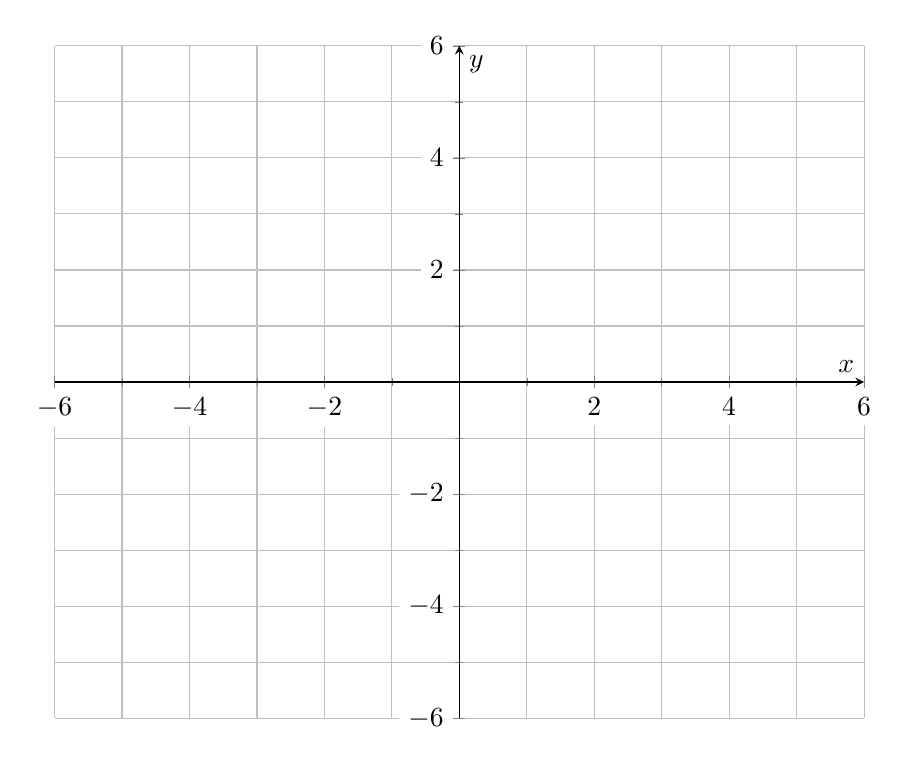
\begin{tikzpicture}
	\begin{axis}[
	grid=both,
	scale=1.5,
	minor tick num=1,
	axis lines=center,
	xmax=6,xmin=-6,
	ymax=6,ymin=-6,
	xlabel=$x$,ylabel=$y$,
	ticklabel style={fill=white},
	]	
	\end{axis}	
	\end{tikzpicture}		
%\end{center}
\clearpage\Question Complete the table of values for the function $g (x) =x^{3} -x$ and sketch the graph
\begin{multicols}{2}
	\begin{tabular}{cc}\toprule
		$x$  & $g (x) =x^3-x$  \\
		\midrule
		$ -1.5$  & \\
		\midrule
		$ -1$  &  \\
		\midrule
		$ -0.5$  &  \\
		\midrule
		$0$  &  \\
		\midrule
		$0.5$  &  \\
		\midrule
		$1$  &  \\
		\midrule
		$1.5$  &  \\
		\bottomrule
	\end{tabular}
	\columnbreak
	\begin{center}
		%blank graph here
		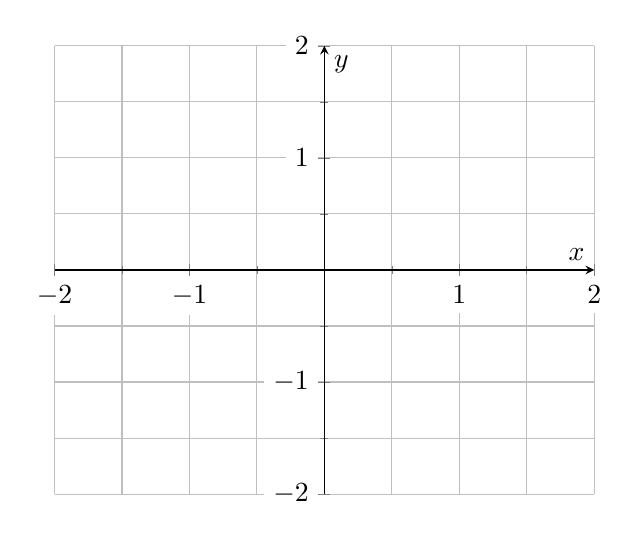
\begin{tikzpicture}
		\begin{axis}[
		grid=both,
		minor tick num=1,
		axis lines=center,
		xmax=2,xmin=-2,
		ymax=2,ymin=-2,
		xlabel=$x$,ylabel=$y$,
		ticklabel style={fill=white},
		]	
		\end{axis}	
		\end{tikzpicture}		
	\end{center}
\end{multicols}
\Question Graph the three functions on a common screen using \desmos. How are the graphs related? 
\begin{tasks}
	\task 	$y =x^{2} ,\text{\quad \quad }y = -x^{2} ,\text{\quad \quad }y =x^{2} \sin  x$  %{L4SZ2818}
	\task   $y =e^{x} ,\text{\quad \quad }y = -e^{x} ,\text{\quad \quad }y =e^{x} \sin  5 \pi  x$ %{L4SZ2819}
\end{tasks}
\Question \begin{tasks}(2)\task Sketch the piece-wise function:\\
\[
f(x) = \begin{cases} 
0 & \mbox{for }x<-2 \\ 
2 & \mbox{for } x>2 \\ 
x& \mbox{for }-2\leq x \leq 2 \\
\end{cases}
\]
\task Write the equation of the function:\\
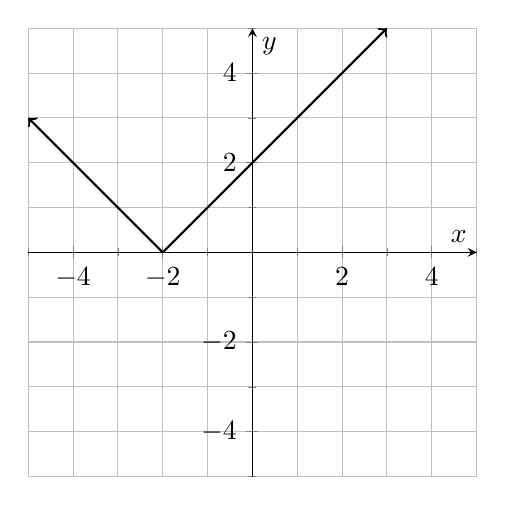
\begin{tikzpicture}
\begin{axis}[grid=both,
scale=1,
unit vector ratio=1 1,
ymin=-5,ymax=5,
xmin=-5,xmax=5,
minor tick num=1,
axis lines = middle,
xlabel=$x$,
ylabel=$y$,
]
\addplot[->,domain=-2:3,samples=50,smooth,thick,black] {x+2};
\addplot[<-,domain=-5:-2,samples=50,smooth,thick,black] {-x-2};
%\draw[step=1,gray,thin,xshift=0cm,yshift=0cm] (0,0) grid (15,15);
\end{axis}
\end{tikzpicture}%$y=|x+2| $
\end{tasks}
\end{Exercise}%functions
\begin{Answer}[ref={ex12}]%functions

\Question %If $f (x) =x^{2}$ and $g (x) =x^{3}$ evaluate
\begin{tasks}
	\task 	 $4$
	\task    $4$	
	\task 	 $27$
	\task    $64$
\end{tasks}

\Question $79.4 \mathrm{m}^{3}$

\Question %Sketch the following graphs (without using Desmos).
\begin{tasks}
	\task 	 $y=4x-4$
	\task    $2y=\frac{x}{3}+1$	
	\task 	 $y =x^{2} -3$ 
	\task    $y =-(x+1)^{2}$ 
\end{tasks}

\Question %Find the $x$ and $y$ intercepts for the graph of $y =x^{2} -3$}%
$x-$intercepts $1.73$ and $ -1.73$ and $y-$intercept $ -3$

\Question %Use the grid provided to answer the following questions. **INSERT GRID HERE**
\begin{tasks}
\task 	 Show the points $A \left (3 ,5\right )$ and $B \left ( -2 , -5\right )$ on\\ the graph.%
\task    $2$	
\task 	$y =2 x -1$ 
\task  $y =2 x +7$
\task  draw a line with a slope of $\frac{4}{5}$
\end{tasks}

\Question Table of Values\smallskip\\% for the function $g (x) =x^{3} -x$ and sketch the graph\vspace{0.5cm} \\\relax
\begin{tabular}{cc}\toprule
	$x$  & $g (x) =x^3-x$  \\
	\midrule
	$ -1.5$  & $ -1.875$  \\
	\midrule
	$ -1$  & $0$  \\
	\midrule
	$ -0.5$  & $0.375$  \\
	\midrule
	$0$  & $0$  \\
	\midrule
	$0.5$  & $ -0.375$  \\
	\midrule
	$1$  & $0$  \\
	\midrule
	$1.5$  & $1.875$  \\
	\bottomrule
\end{tabular}
\Question %Graph the three functions on a common screen using \desmos. How are the graphs related? 
\begin{tasks}
	\task 	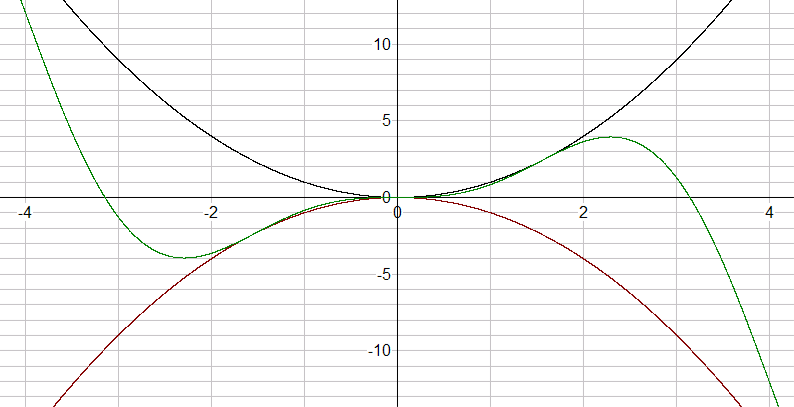
\includegraphics[width=5cm]{L4SZ2818}\\
	\task   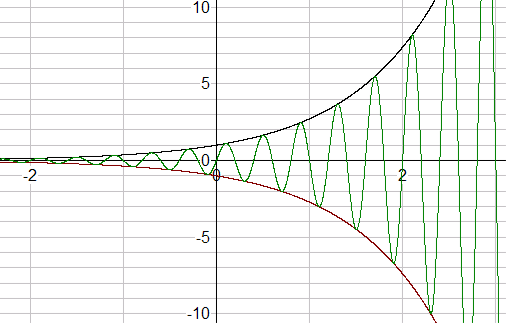
\includegraphics[width=5cm]{L4SZ2819}\\
\end{tasks}
\Question 
	\begin{tasks}\task
	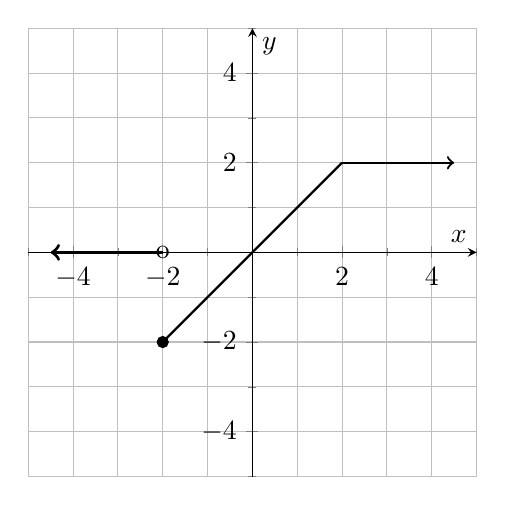
\begin{tikzpicture}
	\begin{axis}[grid=both,
	scale=1,
	unit vector ratio=1 1,
	ymin=-5,ymax=5,
	xmin=-5,xmax=5,
	minor tick num=1,
	axis lines = middle,
	xlabel=$x$,
	ylabel=$y$,
	]
	\addplot[<-,domain=-4.5:-2,samples=50,smooth,very thick,black] {0};
	\addplot[->,domain=2:4.5,samples=50,smooth,thick,black] {2};
	\addplot[-,domain=-2:2,samples=50,smooth,thick,black] {x};\\
	\addplot[mark=*] coordinates {(-2,-2)};
	%dirty hack to get an open dot!
	\node [circle,inner sep=0.5pt] at (axis cs:-2,0) {o};
	\end{axis}
	\end{tikzpicture}
	\task $y=|x+2| $
	\end{tasks}
\end{Answer}%functions

%-------------------------------------------------------------------
% POLYNOMIALS
%-------------------------------------------------------------------
\begin{Exercise}[title={Polynomials},label=ex13]
	\Question What is the degree of the polynomial?
	\begin{tasks}(2)
		\task 	 $y=x^2$%{$2$}\\
		\task    $4x^3-2x^2+6=0$%{$3$}\\
		\task 	 $a^{99}-99a^2=-99$%{$99$}
		\task    $ey^4- ey^3+ ey^2-ey^1+e$%{4}
	\end{tasks}
	
	\Question Are the following considered polynomials?
	\begin{tasks}(4)
		\task 	 $\pi$%{No, there is no variable term}
		\task 	 $\pi^x$%{No, a variable in the exponent is an \textit{exponential} equation}
		\task    $Ax^2+Bx+C$%{Yes}
		\task    $4x^3-2x^{\frac{3}{2}}+1=0$%{No, the powers must be integers}
	\end{tasks}

	\Question Make up your own polynomials of degree 1,2,3, and 4.
\end{Exercise}%polynomials
\begin{Answer}	[ref={ex13}]
	\Question %What is the degree of the polynomial?
\begin{tasks}
	\task 	 $2$
	\task    $3$
	\task 	 $99$
	\task    $4$
\end{tasks}

\Question %Are the following considered polynomials?
\begin{tasks}
	\task 	 No, there is no variable term
	\task 	 No, a variable in the exponent is an \\\textit{exponential} equation
	\task    Yes
	\task    No, the powers must be integers
\end{tasks}

%\Question %Make up your own polynomials of degree 1,2,3, and 4.	
\end{Answer}%polynomials
	
%-------------------------------------------------------------------
% systemsOfEquations
%-------------------------------------------------------------------
\begin{Exercise}[title={Systems of Equations},label=ex14]
	\Question Solve the system of equations graphically. For the non-linear ones you may want to use \desmos.
		\begin{tasks}(2)
			\task 	
			\begin{tabular}{r@{}l}
			$y$&$=2x+6$\\%$(-$\frac{1}{3},5$\frac{1}{3})$
			$y$&$=-x+5$
			\end{tabular}\medskip 
			\task  
			\begin{tabular}{r@{}l}
			$\frac{3y}{4}+1$&$=x$\\%$(0.571,-0.571)$
			$-x$&$=y$
			\end{tabular}   
			\task 
			\begin{tabular}{r@{}l}%infinite solutions
				$-x+\frac{1}{2}y\,$&$=-5$\\
				$2x-y\,$&$=10$
			\end{tabular}\medskip	 
			\task    
			\begin{tabular}{l}
				$\frac{x^2}{9}+\frac{y^2}{18}=1$\\%$\left (1.23 ,3.87\right ) ,\left ( -0.35 , -4.21\right )$
				$y=-x^2+6x-2$
			\end{tabular}  
		\end{tasks}
		\Question Solve the system using substitution.
		\begin{tasks}(2)
			\task 	
			\begin{tabular}{l}
				$x-y=2$\\%$(3,1)$
				$2x+3y=9$
			\end{tabular}\medskip  
			\task    	
			\begin{tabular}{l}
				$2x-3y=12$\\%no solutions
				$-x+\frac{3}{2}y=4$
			\end{tabular} 
			\task 	 
			\begin{tabular}{l}
				$x+y=8$\\%$(18.29,-10.29)$
				$y=-8-\frac{x}{8}$
			\end{tabular} 
			\task    
			\begin{tabular}{l}
				$x+y^2=0$\\%$(-25,5)$, and $(-25,-5)$
				$2x+5y^2=75$
			\end{tabular} 
		\end{tasks}
\Question Solve the system by eliminating a variable.
		\begin{tasks}(2)
			\task 	 
			\begin{tabular}{r@{}l}%$(1,2)$
				$x+2y\,$&$=5$\\
				$2x+3y\,$&$=8$
			\end{tabular}\medskip	
			\task   
			\begin{tabular}{r@{}l}%$(-3,4)$ and $(3,4)$
				$x^2-2y\,$&$=1$\\
				$x^2+5y\,$&$=29$
			\end{tabular} 
			\task
			\begin{tabular}{r@{}l}%$(-2,-1)$ , $(-2,1)$ , $(2,-1)$ , $(2,1)$
				$3x^2-\phantom{1}y^2\,$&$=11$\\
				$\phantom{1}x^2+4y^2\,$&$=8$
			\end{tabular} 	 
			\task    
			\begin{tabular}{r@{}l}%$(-1.5,0)$
				$12x+15y\,$&$=-18$\\
				$2x+\phantom{1}5y\,$&$=-3$
			\end{tabular} 	 
		\end{tasks}
\end{Exercise}%SystemsofEquations

\begin{Answer}[ref={ex14}]	
\Question %Solve the system of equations graphically
\begin{tasks}
	\task 	$(-\frac{1}{3},5\frac{1}{3})$
	\task   $(0.571,-0.571)$ 
	\task 	infinite solutions 
	\task   $\left (1.23 ,3.87\right ) ,\left ( -0.35 , -4.21\right )$ 
\end{tasks}
\Question %Solve the system using substitution
\begin{tasks}
	\task 	 $(3,1)$
	\task    no solution; parallel lines
	\task 	 $(18.29,-10.29)$
	\task    $(-25,5)$, and $(-25,-5)$
\end{tasks}
\Question %Solve the system by eliminating a variable
\begin{tasks}
	\task 	 $(1,2)$
	\task    $(-3,4)$ and $(3,4)$
	\task 	 $(-2,-1)$ , $(-2,1)$ , $(2,-1)$ , $(2,1)$
	\task    $(-1.5,0)$
\end{tasks}
\end{Answer}%SystemsofEquations

%-------------------------------------------------------------------
% word problems
%-------------------------------------------------------------------
\begin{Exercise}[title={Word Problems},label=ex15]
	\Question A rectangle has an area of $180\text{ cm}^{2}$ and a perimeter of $54 \mbox{cm}$. What are its dimensions? 
	\Question The admission fee at an amusement park is $ \$1.50$ for children and $ \$4.00$ for adults. On a certain day, $2200$ people entered the park and the admission fees collected totalled $ \$5050$. How many children and how many adults were admitted? 
	\Question A woman keeps fit by bicycling and running every day. One Monday she spends $\frac{1}{2} \mbox{h}$ at each activity and covers a total of $12\frac{1}{2} \mbox{mi}$. On Tuesday she runs for $12 \mbox{min}$ and cycles for $45 \mbox{min}$, covering a total of $16 \mbox{mi}$. Assuming her running and cycling speeds don't
	change from day to day, find these speeds.
	\Question A customer
	in a coffee shop purchases a blend of two coffees: Kenyan, costing $ \$3.50$ a pound, and Sri Lankan, costing $ \$5.60$ a pound. He buys $3 \mbox{lb}$ of the blend, which costs him $ \$11.55$. How many pounds of each kind went into the mixture?
\end{Exercise}%word problems
\begin{Answer}[ref={ex15}]		
	\Question $12 \mbox{cm}$ by $15 \mbox{cm}$
	\Question The number of children admitted was 1500\\ and the number
	of adults was 700.
	\Question Run $5 mi/\mbox{h}$, cycle $20 mi/\mbox{h}$ 
	\Question $2.5$ pounds of Kenyan coffee and $0.5$ pounds\\ of Sri Lankan coffee should be mixed. 
\end{Answer}%word problems

%-------------------------------------------------------------------
% END exercises
%-------------------------------------------------------------------


